\documentclass{article}
\usepackage{natbib}
\usepackage{graphicx}
\usepackage{amsmath}
\usepackage{multirow}
\usepackage{graphicx}
\usepackage[letterpaper, left=1in, right=1in, top=1in, bottom=1in]{geometry}

\title{Optimizing Document Clustering through Correlation-Driven Cluster Formation}
\author{Suraj Kashyap\textsuperscript{1} and Uttam Mahata\textsuperscript{1}}
\date{}

\begin{document}

\maketitle

\textsuperscript{1} Department of Computer Science and Technology, Indian Institute of Engineering Science and Technology, Shibpur, Howrah, India

\section*{Abstract}
Document clustering is a vital component in organizing extensive datasets for efficient information retrieval and analysis. This paper presents an innovative method for enhancing clustering algorithms by dynamically adjusting parameters based on correlation thresholds. Utilizing Natural Language Processing for textual data preprocessing, the study evaluates the approach using established clustering metrics. Results demonstrate the method's adaptability to diverse datasets, yielding notable improvements in clustering accuracy and efficiency. The identified optimal threshold values offer valuable insights for parameter selection, making this approach a significant contribution to clustering optimization. The findings hold promise for advancing the practicality of clustering algorithms in various data-driven applications, particularly in domains like data science and machine learning.

\section*{Keywords}
Information Retrieval, Threshold Value, Spearman Correlation Coefficient, Jaccard Coefficient, Cluster Formation, Error Calculation, Elbow Method, Comparative Analysis, K-Means Algorithm, Affinity Propagation, Gaussian Mixture Model, Agglomerative Clustering, Silhouette Score, Davies-Bouldin Index, Calinski Harabasz Score, Adjusted Rand Score, Normalized Mutual Information Score

\section{Introduction}
In the ever-expanding digital content landscape, effective document clustering plays a pivotal role in organizing extensive datasets for efficient information retrieval and analysis. This research paper presents an innovative approach to document clustering optimization through correlation-driven techniques. The methodology integrates a sophisticated preprocessing pipeline, encompassing tokenization, lemmatization, and TF-IDF vectorization, laying the foundation for a dynamic optimization process.

Document clustering is a crucial task in information retrieval and text mining. In this literature review, we explore various optimization-driven and descriptive document clustering approaches proposed by researchers.
Jensi and Jiji \cite{jensi2014survey} conducted a survey on optimization approaches to text document clustering. They compared the performance of techniques such as K-means, Fuzzy C-means, and Genetic Algorithm on different datasets, highlighting the dependency on both the dataset and the optimization technique used. Kayest and Jain \cite{kayest2022optimization} proposed an optimization-driven cluster-based indexing and matching approach for document retrieval. Their method, outperforming traditional indexing techniques, utilized clustering to group similar documents and an indexing technique for efficient retrieval. Brockmeier et al. \cite{brockmeier2018self} introduced a self-tuned descriptive document clustering approach using a predictive network. By employing a neural network to predict the optimal number of clusters, they demonstrated improved performance compared to traditional clustering algorithms. Tolner et al. \cite{9668337} proposed a clustering approach based on LDA topic modeling for business organizations. They used a topic modeling algorithm to extract topics from documents, followed by a clustering algorithm for grouping. This approach exhibited superior performance compared to traditional methods. Alharbi et al. \cite{alharbi2021enhancing} enhanced topic clustering for Arabic security news using k-means and topic modeling. Their method showcased improved performance compared to traditional clustering algorithms. Wahid and Hassini \cite{wahid2022literature} conducted a literature review on correlation clustering, providing a cross-disciplinary taxonomy and analyzing developments from 1992 to 2020. The authors presented mathematical formulations and solution approaches, identified gaps, and proposed future research directions.

Our work makes the following contributions:
\begin{itemize}
    \item Dataset Preparation
    \item Data Preprocessing
    \item Cluster Formation
    \item Correlation-based Thresholding
\end{itemize}
In light of this rich literature landscape, our research contributes by introducing a correlation-driven optimization approach to document clustering. The ensuing sections will delve deeper into the methodology, experimental setups, and comparative analyses, positioning our approach within the broader context of advancements in clustering algorithms for various data types. Basic steps followed here is shown below: 
\begin{figure}[ht]
    \centering
    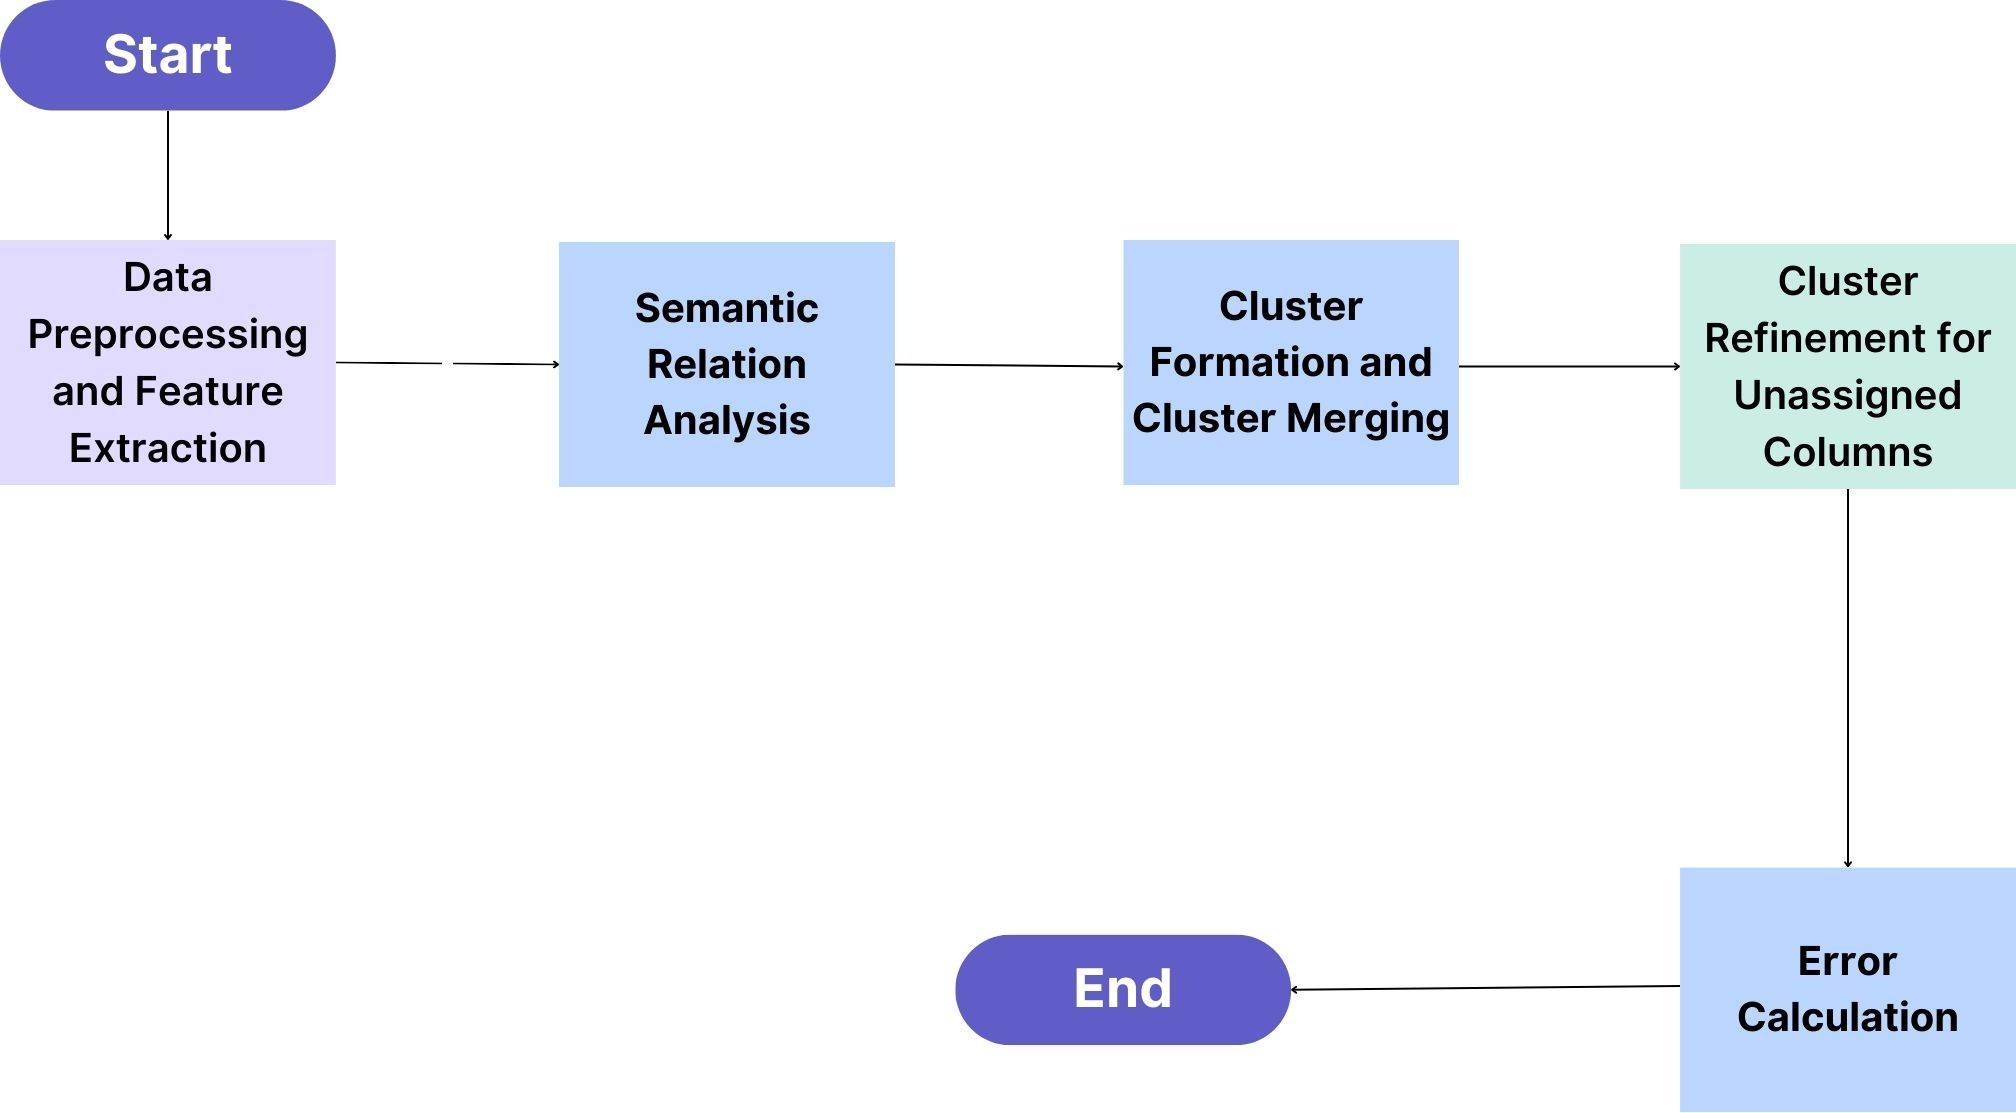
\includegraphics[width=1\linewidth]{flow.jpg}
    \caption{Flow Diagram for Steps}
    \label{fig:graph4}
\end{figure}

% Add more sections as needed
\section{Methodology}
The Threshold-based Correlation Clustering (TBCC) methodology orchestrates a systematic process for optimizing clusters using TF-IDF vectors' correlation matrix. Beginning with data preprocessing involving tokenization and lemmatization, the methodology ensures a standardized and cleaned dataset. TF-IDF vectors are then generated, providing the foundation for Spearman correlation-based correlation matrix calculation. The clustering process identifies cohesive semantic groups by considering above-average correlations. The Jaccard coefficient is employed to quantify overlap between clusters, guiding the iterative optimization through threshold-based merging. Convergence is reached when no pair of clusters exhibits a maximum correlation above a specified threshold. To enhance clustering quality, an iterative refinement process addresses unassigned columns.
In essence, TBCC systematically refines clusters, emphasizing semantic coherence and distinctiveness within the dataset, making it a robust approach for uncovering meaningful relationships in textual data.
\subsection{Data Preprocessing and Feature Extraction}
The preprocessing phase involves eliminating stop words and applying stemming techniques to refine the text database. Stop words, such as 'a,' 'an,' 'in,' 'the,' are excluded during searches, streamlining the retrieval of meaningful results. Simultaneously, stemming reduces words to their root form, enhancing comparability during observations. The resulting dictionary words serve as the foundation for subsequent feature extraction, ensuring a more precise and optimized text dataset for advanced analyses within the TBCC methodology.

 Feature extraction is pivotal in transforming textual data into quantifiable features for meaningful analysis. It involves generating TF-IDF (Term Frequency-Inverse Document Frequency) vectors, a numerical representation that gauges the importance of each term within a document relative to the entire dataset \cite{ref1}. The weight assigned by TF-IDF amplifies with a term's prevalence in a document, underscoring its significance, and diminishes for ubiquitous terms. The Inverse Document Frequency calculates the importance of rarely occurring words. The TF-IDF is expressed as:
\[ \text{TF-IDF}(A, B, E) = S(A, B) \times T(A, E) \]

where \( S(A, B) \) is the Term Frequency (TF), \( T(A, E) \) is the Inverse Document Frequency (IDF), \( A \) denotes words, \( B \) denotes each document, and \( E \) denotes the collection of documents. The IDF formula is:
\[ \text{IDF}(A, E) = \log\left(\frac{N}{1 + \text{df}(A, E)}\right) \]

Here, \( A \) is the term, \( E \) is the document collection, \( N \) is the total number of documents in \( E \), and \( \text{df}(A, E) \) is the document frequency of term \( A \) in \( E \).



 \subsection{Semantic Relationship Analysis}

The procedure for semantic relationship analysis commences with the calculation of the correlation matrix ($C$) derived from TF-IDF vectors. Spearman's Rank Correlation Coefficient ($\rho$) is employed to robustly measure monotonic relationships between words, ensuring a comprehensive understanding of semantic associations.
\[ \rho = 1 - \frac{6 \sum d_i^2}{n(n^2 - 1)} \]

where $d_i$ is the difference between the ranks of corresponding TF-IDF values for the $i$-th pair of words, and $n$ is the number of pairs.

This step guarantees that the correlation matrix captures both linear and potential nonlinear dependencies, enriching the semantic insights \cite{arsov2019measure}.
\subsection{Cluster Formation and Cluster Merging}

The Cluster Formation step plays a pivotal role in capturing semantic coherence among words by creating groups with above-average correlations. The process begins with a row-wise calculation, evaluating the average correlation (\( \text{Average Corr}_k \)) for each word. This provides a measure of each word's overall association with others in the dataset. Clusters are then formed by selecting words with individual column-wise average correlation values (\( Corr_{ki} \)) surpassing the global average. The criterion for inclusion in a cluster is that the individual correlation values must exceed the specified threshold (\( T \)).
\[ Cluster_k = \{word_i \mid Corr_{ki} > \text{Average Corr}_k > T\} \]
This clustering strategy emphasizes grouping words with stronger-than-average semantic relationships, laying the foundation for subsequent optimization steps in the TBCC methodology.


Following Cluster Formation, the methodology proceeds to calculate the Jaccard Coefficient between pairs of clusters. The Jaccard Coefficient quantifies the degree of overlap between clusters and serves as a meaningful metric for assessing the distinctiveness and coherence of the formed semantic clusters. The Jaccard Coefficient between two clusters \( A \) and \( B \) is computed as: \[ \text{Jaccard Coefficient}(A, B) = \frac{|A \cap B|}{|A \cup B|} \]

This measure provides valuable insights into the similarity between clusters, contributing to the evaluation of the overall quality and cohesion of the formed semantic groups. The evaluation is informed by multiple sources, including the research conducted by Irani et al. \cite{irani2016clustering}, which discussed clustering techniques and the similarity measures used in clustering.
The TBCC methodology iteratively optimizes clusters by merging those with Jaccard coefficients above the specified threshold \( T \). This iterative process ensures the formation of meaningful and distinct clusters. The merging criterion is defined as:
\[ \text{Merge Cluster } A \text{ and Cluster } B \text{ if } \text{Jaccard Coefficient}(A, B) \geq T \]

This approach systematically refines clusters, producing semantically cohesive clusters representing distinct concepts or themes within the dataset.


The optimization process within TBCC continues until convergence, ensuring that no pair of clusters exhibits a maximum correlation above the specified threshold \( T \). The convergence criteria can be expressed as:

\[ \max(C_{ij}) < T \]

This condition signifies that the optimization process converges when the maximum correlation between any pair of clusters falls below the threshold.
To refine the clustering results, an iterative procedure assesses columns initially unassigned to any clusters. The algorithm identifies clusters with a single-column representation and evaluates the relationships between unassigned columns and those clusters. The refinement process contributes to the overall quality of clustering by addressing any unassigned or outlier columns within the dataset. These steps in the TBCC methodology collectively contribute to the systematic optimization of clusters, producing semantically cohesive and distinct groupings within the textual data.
\subsection{Cluster Refinement for Unassigned Columns}
To refine the clustering results, an iterative procedure assesses columns initially unassigned to any clusters. The algorithm identifies clusters with a single column representation and evaluates the relationships between unassigned columns and those clusters.

\textbf{Refinement Criteria}: For each unassigned column, it assesses its relationship with columns in clusters with a single representation. A refinement criterion stipulates that if at least 75 percent of columns within the same original cluster support the assignment of an unassigned column, it is reassigned to that cluster.

\textbf{Assignment Process}: If the criteria are met, the unassigned column is reassigned to the identified cluster. If the criteria are not met, the column is treated as a singleton cluster.


\section{Experimental Setup}
\subsection{Dataset Description}
We employed a dataset consisting of 200 questions across four topics: Biotechnology, Database Management System (DBMS), Network and Networking, and Climate Change. Each topic comprised 50 questions. The selection of topics was arbitrary, ensuring no specific influence on the clustering algorithm's functionality. The initial phase involved transforming raw text data for clustering, including tokenization, lemmatization, stopword and punctuation filtering, and TF-IDF vectorization. This process resulted in numerical vectors, forming the foundation for evaluating the clustering algorithm's performance and comparing it against established methods.
\subsection{Experiment Conduct}

The experiments were conducted using the TBCC methodology, as detailed in the previous methodology section. The implementation utilized the following software and tools: Python, Scikit-learn, NumPy, Pandas, NLTK for tokenization and lemmatization. The implementation followed the steps outlined in the TBCC methodology, encompassing data preprocessing, TF-IDF vectorization, semantic relationship analysis, cluster formation, evaluation of cluster overlap using the Jaccard Coefficient, and threshold-based cluster merging.

\subsection{Parameter Settings}

In our experiment, the focus was on determining the optimum threshold value for our custom clustering algorithm, a critical factor influencing the strength of semantic correlations between words and, consequently, the formation of clusters. The threshold values were systematically varied from 0.2 to 0.3 in increments of 0.01 for each iteration. For each threshold value, we calculated the corresponding number of clusters and the associated error. The process involved the following steps:

\textbf{Threshold Variation: } In clustering algorithms, particularly within our methodology, the computation of centroids plays a crucial role in unraveling and characterizing the inherent qualities of clusters. The centroid (\( \text{Centroid}_k \)) for a specific cluster (\( \text{Cluster}_k \)) is calculated using the equation:

\[ \text{Centroid}_k = \frac{\sum_{i \in \text{Cluster}_k} \text{TF-IDF}_i}{\text{Number of Documents in Cluster}_k} \]
\begin{figure}[ht]
    \centering
    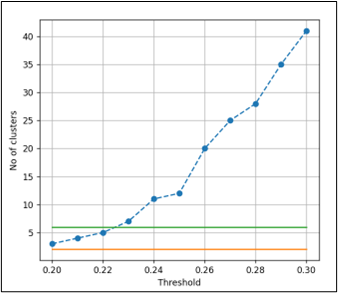
\includegraphics[width=0.4\linewidth]{Graph1.png}
    \caption{Caption for Graph 1}
    \label{fig:graph1}
\end{figure}


The computed centroids serve as fundamental metrics, facilitating a comprehensive analysis of central tendencies and prevalent themes within individual clusters. In our study, we systematically varied threshold values from 0.2 to 0.3. For each threshold value, our custom clustering algorithm was applied to the dataset, yielding distinct clustering arrangements. This approach allowed us to explore the impact of different threshold levels on the resulting cluster configurations.

\textbf{Identification of Optimum Threshold: } The elbow method, a widely employed technique, entails plotting the rate of change in error against various threshold values. The optimal threshold is discerned at the juncture where the rate of error reduction experiences a significant slowdown, resembling the characteristic bend of an elbow in the plot. This threshold value strikes a balance between cluster coherence (minimizing error) and meaningfulness, ensuring a reasonable number of clusters.
The assessment of clustering quality hinges on accurate error calculation. Our methodology adopts the Root Mean Square (RMS) difference between document TF-IDF vectors and their corresponding cluster centroids.
The RMS calculation for a document-cluster pair is given by:
\[ \text{RMS(Document, Cluster)} = \sqrt{\frac{\sum_{i=1}^n (x_i - \bar{x})^2}{n}} \]
where \( n \) is the dimensionality of the vectors, \( x_i \) represents individual vector components, and \( \bar{x} \) denotes the mean.
Cluster-wise error (\( E_{\text{cluster}} \)) is the average RMS value across all documents in a cluster:
\[ E_{\text{cluster}} = \frac{\sum_{j=1}^m \text{RMS(Document}_j, \text{Cluster})}{m} \]
where \( m \) is the number of documents in the cluster.
Global error (\( E_{\text{global}} \)) is the average of cluster-wise errors across all clusters:
\[ E_{\text{global}} = \frac{\sum_{k=1}^K E_{\text{cluster}_k}}{K} \]
where \( K \) is the total number of clusters. This comprehensive error assessment framework ensures a nuanced evaluation of clustering effectiveness.


\begin{figure}[ht]
    \centering
    \begin{minipage}{0.45\textwidth}
        \centering
        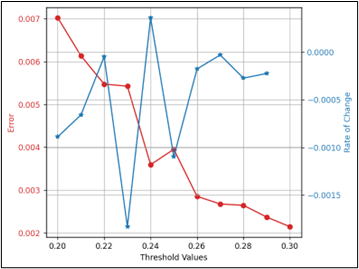
\includegraphics[width=\linewidth]{Graph2.png}
        \caption{Caption for Graph 2}
        \label{fig:graph2}
    \end{minipage}
    \hfill
    \begin{minipage}{0.45\textwidth}
        \centering
        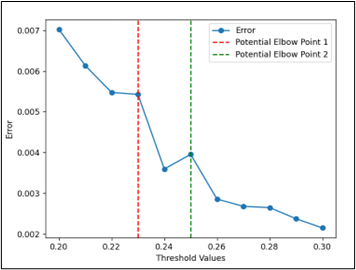
\includegraphics[width=\linewidth]{Graph3.png}
        \caption{Caption for Graph 3}
        \label{fig:graph3}
    \end{minipage}
\end{figure}

\section{Results and Discussions}
The experimental findings offer valuable insights into the performance of the Custom Clustering Algorithm in contrast to conventional methods. By establishing a fixed optimum threshold, we ensured the stability of subsequent analyses, providing a consistent basis for evaluation. The performance assessment involved a meticulous comparison of the custom algorithm with other clustering methods, particularly at the optimal cluster number—set at four to align with the original topics of Biotechnology, DBMS, Network and Networking, and Climate Change.

This deliberate parameterization strategy served a dual purpose: first, it optimized the algorithm's performance within its intrinsic settings, and second, it facilitated an insightful evaluation of its adaptability across specific scenarios. The consideration of the original cluster number further enhanced the relevance and applicability of the assessment, contributing to a holistic understanding of the algorithm's capabilities.

\subsection{Computational Efficiency and Comparative Analysis}
The custom clustering algorithm demonstrates efficient performance, with clustering, centroid and error calculation taking approximately 3-4 seconds. When determining the optimum number of clusters using the elbow method, the algorithm displayed superior performance with threshold values of 0.23 and 0.25 compared to standard clustering methods. Despite the inherent challenge of setting an optimal threshold, the algorithm showcased better Silhouette scores, Calinski Harabasz scores, and Adjusted Rand Scores. The Normalized Mutual Information Score also demonstrated the algorithm's effectiveness in capturing meaningful semantic relationships. The Custom Clustering Algorithm, with threshold values of 0.23 and 0.25, demonstrated competitive performance compared to standard clustering algorithms such as KMeans, Affinity Propagation, Gaussian Mixture, and Agglomerative Clustering. The Davies-Bouldin index, Silhouette score, Calinski Harabasz score, Adjusted Rand Score, and Normalized Mutual Information Score were used as metrics for evaluation.
\begin{table}[ht]
    \centering
    \resizebox{\textwidth}{!}{
        \begin{tabular}{cccccc}
            \hline
            Model & Davies-Bouldin Index & Silhouette Score & Calinski Harabasz Score & Adjusted Rand Score & Normalized Mutual Info Score \\
            \hline
            Custom Clustering Algorithm (0.23) & 1.0755 & 0.2502 & 63.9523 & 0.8651 & 0.8684 \\
            Custom Clustering Algorithm (0.25) & 0.8524 & 0.2445 & 122.0241 & 0.8721 & 0.8694 \\
            KMeans & 2.2553 & 0.1106 & 124.9375 & 0.6236 & 0.7595 \\
            Affinity Propagation & 1.3178 & 0.2664 & 297.9176 & 0.8666 & 0.8675 \\
            Gaussian Mixture & 2.8988 & 0.0506 & 122.9254 & 0.4891 & 0.6936 \\
            Agglomerative Clustering & 2.0598 & 0.1198 & 128.7157 & 0.5726 & 0.7294 \\
            \hline
        \end{tabular}
    }
    \caption{Optimum Number of Clusters}
    \label{tab:my_label}
\end{table}

\begin{figure}[ht]
    \centering
    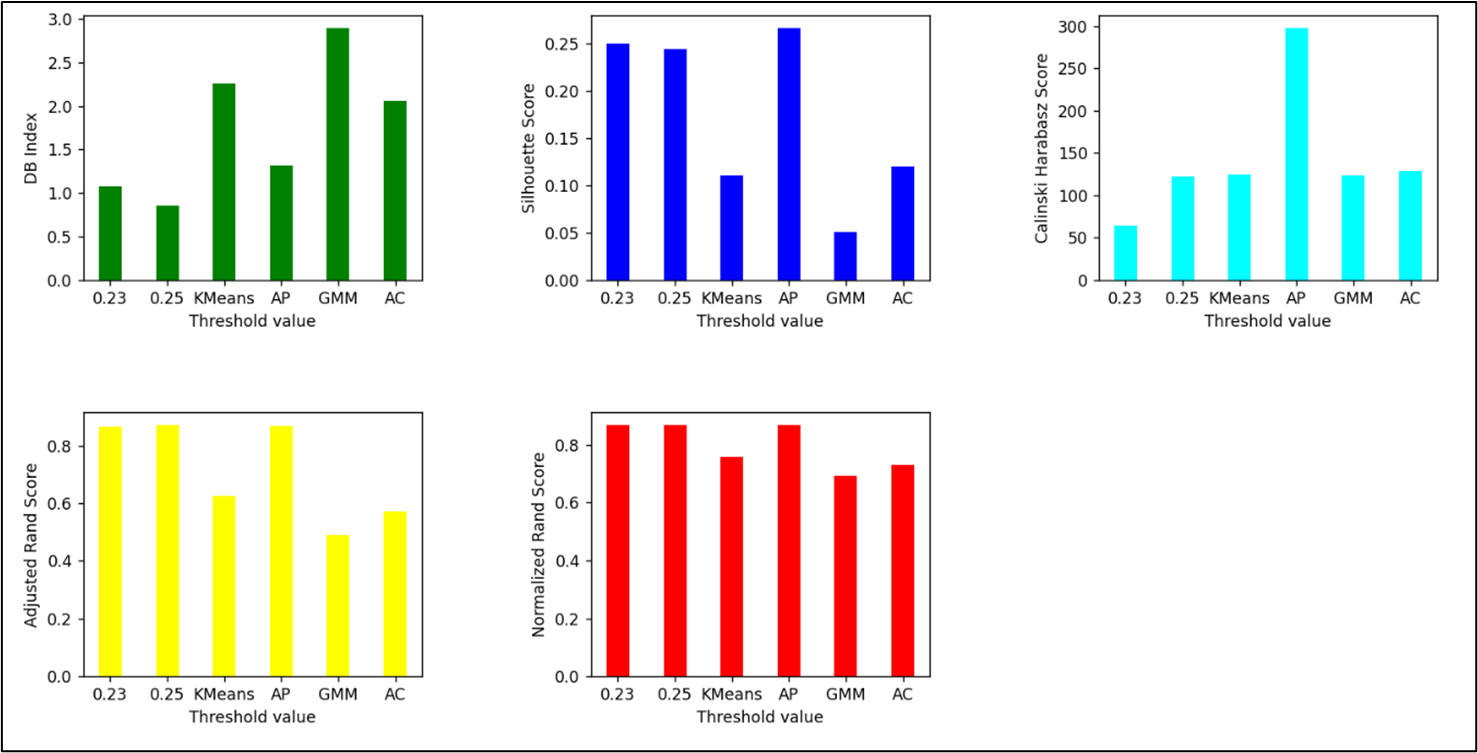
\includegraphics[width=1\linewidth]{Graph4.png}
    \caption{Caption for Graph 4}
    \label{fig:graph4}
\end{figure}


\begin{table}[ht]
    \centering
    \resizebox{\textwidth}{!}{
        \begin{tabular}{cccccc}
\hline
        Model & Davies-Bouldin index & Silhouette Score & Calinski Harabasz score & Adjusted Rand Score & Normalized Mutual Info Score \\
        \hline
        Custom Clustering Algorithm (0.23) & 1.0755 & 0.2502 & 63.9523 & 0.8651 & 0.8684 \\
        Custom Clustering Algorithm (0.25) & 0.8524 & 0.2445 & 122.0241 & 0.8721 & 0.8694 \\
        KMeans & 1.0535 & 0.4173 & 318.6811 & 0.6050 & 0.7224 \\
        Affinity Propagation & 1.3178 & 0.2664 & 297.9176 & 0.8666 & 0.8675 \\
        Gaussian Mixture & 1.4542 & 0.2545 & 261.868 & 0.8390 & 0.8438 \\
        Agglomerative Clustering & 1.0346 & 0.4144 & 314.3739 & 0.6346 & 0.7512 \\
        \hline
        \end{tabular}
    }
    \caption{Optimum Number of Clusters}
    \label{tab:my_label}
\end{table}
\begin{figure}[ht]
    \centering
    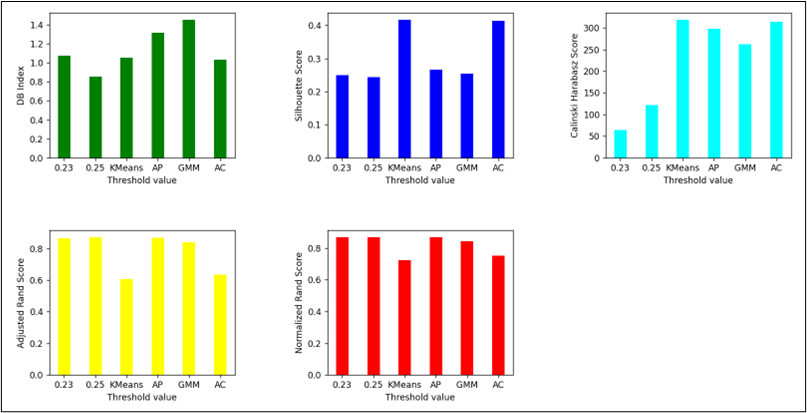
\includegraphics[width=1\linewidth]{Graph5.png}
    \caption{Caption for Graph 4}
    \label{fig:graph4}
\end{figure}


The results indicate that the proposed algorithm achieved lower Davies-Bouldin indices, higher Silhouette scores, and competitive Calinski Harabasz scores. The Adjusted Rand Score and Normalized Mutual Information Score also highlight the algorithm's ability to form clusters with meaningful semantic associations.

\section{Conclusion}
The algorithm's strengths lie in its adaptability to varying document relationships through dynamic correlation-based optimization. By leveraging semantic relationships, the algorithm creates cohesive and meaningful clusters. However, a potential limitation is the sensitivity to the choice of the correlation threshold, which warrants further exploration.The Custom Clustering Algorithm holds promise in various applications where document organization and extraction of semantic patterns are crucial. Its ability to dynamically adjust to document relationships makes it suitable for datasets with diverse content and varying semantic associations.
Future research could explore mechanisms for automated selection of correlation thresholds based on the dataset's characteristics. Additionally, scalability and robustness assessments on larger and more diverse datasets could further validate the algorithm's effectiveness.

\bibliographystyle{plain}
\bibliography{references}

\end{document}
